\appendix
\section{Cantilever beam dynamics}

Consider an eVTOL wing with multiple electric motors and rotors mounted along the spar, shown in Fig.~\ref{fig:wing_diagram}. The wing structure is idealized as a cantilever beam with non-structural lumped masses placed along the span, shown in Fig.~\ref{fig:cantilever}. 

\begin{figure}[H]
     \centering
         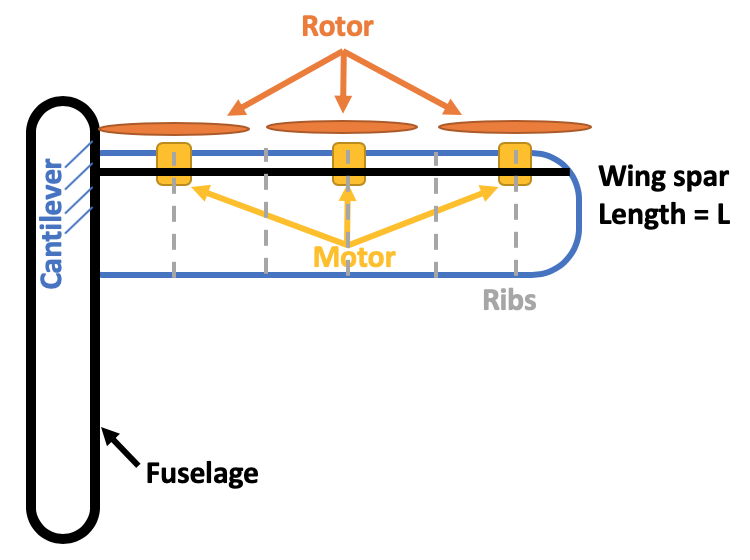
\includegraphics[width=0.7\textwidth]{images/wing_diagram.png}
        \caption{Rotor layout for an example eVTOL wing}
         \label{fig:wing_diagram}
\end{figure}

\begin{figure}[H]
         \centering
         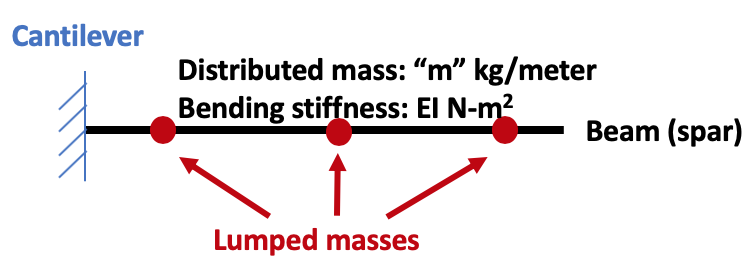
\includegraphics[width=0.7\textwidth]{images/cantilever.png}
        \caption{Idealization of eVTOL wing structure}
         \label{fig:cantilever}
\end{figure}

To expand the generality of the analysis, consider a tapered circular spar running along the length of the wing. The cross-section of the spar is shown in Fig.~\ref{fig:taper_beam}. The tube thickness is equal to $t$, and is uniform along the spar length. The radius of the circular cross-section varies from $r_1$ at the root of the beam to $r_2$ at the tip. The mass per unit span and bending stiffness of the spar is given by 
\begin{align*}
m(x) \quad &= \quad 2 \pi \rho r(x) t \\
EI_{yy}(x) \quad &= \quad E \pi r(x)^3 t
\end{align*}

\begin{figure}
\begin{center}
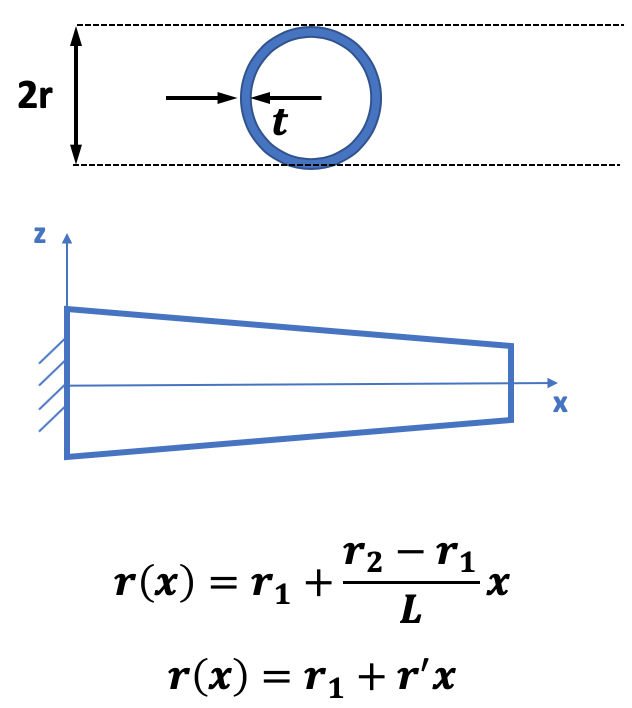
\includegraphics[width=0.45\textwidth]{images/taper_beam.png}
\vspace{-0.1cm}
\caption{Linearly tapered circular spar}
\label{fig:taper_beam}
\end{center}
\end{figure}

The first bending natural frequency is estimated using a Rayleigh-Ritz approximation, with a mode shape set by the static deflection of the cantilever due to a tip-load, i.e.,
\begin{equation}
w''(x) \quad = \quad P (L - x)
\end{equation}
Integrate twice along the span and apply the cantilever boundary condition to obtain the deflected bending slope as 
\begin{equation}
w'(x) \quad = \quad \frac{P}{E\pi t}\left[\frac{a_2}{r(x)^2} \spc+\spc \frac{a_1}{r(x)} \spc+\spc a_0\right]
\end{equation}
The constants are 
\begin{align*}
a_2 \quad =& \quad -\frac{L}{2r'} \spc-\spc \frac{r_1}{2{r'}^2} \\
a_1 \quad =& \quad -\frac{1}{{r'}^2} \\
a_0 \quad =& \quad \frac{L}{2r'r_1^2} \spc-\spc \frac{1}{2{r'}^2 r_1}
\end{align*}
Integrate the bending slope along the span to obtain the deflected mode shape as 
\begin{equation}
w(x) \quad = \quad \frac{P}{E\pi t}\left[b_0 \spc + \spc b_1 x \spc+\spc \frac{b_m}{r(x)} \spc+\spc b_l \log_e r(x)\right]
\end{equation}
The constants are 
\begin{align*}
b_0 \quad =& \quad -\frac{a_2}{r_1 r'} \spc-\spc \frac{a_1}{r'} \log_e(r_1)\\
b_1 \quad =& \quad a_0 \\
b_m \quad =& \quad -\frac{a_2}{r'}  \\
b_l \quad =& \quad \frac{a_1}{r'} 
\end{align*}
\subsection{Potential energy}
The maximum potential energy is given by 
\begin{equation*}
U \quad = \quad \frac{1}{2} \int_0^L \frac{P^2(L-x)^2}{EI_{yy}(x)} dx
\end{equation*}
Substitute for the bending stiffness to obtain 
\begin{equation*}
U \quad = \quad \frac{1}{2} \frac{P^2}{E\pi t} [A + B + C](\lambda) 
\end{equation*}
The term $\lambda$ is the spar taper ratio, given by 
\begin{equation}
\lambda \quad = \quad \frac{r_2}{r_1}
\end{equation}
The sum $A+B+C$ is well-represented by a cubic polynomial in $\lambda$ as 
\begin{equation*}
A+B+C\quad \approx \quad (1.6261 \spc - \spc 0.4826 \lambda \spc + \spc 2.1197 \lambda^2 \spc - \spc 0.5957 \lambda^3) \frac{1}{K^3}
\end{equation*}
The constant $K$ is the inverse of the spar aspect ratio, given by 
\begin{equation}
K \quad = \quad \frac{2 (\frac{t}{c})}{AR_{\rm wing}}
\end{equation}
Here, $\frac{t}{c}$ is the wing thickness to chord ratio, and $AR_{\rm wing}$ is the wing aspect ratio.

\subsection{Kinetic energy}
The maximum kinetic energy of the beam has contributions from three types of masses:
\begin{enumerate}
\item \textbf{Structural masses}: This term deals with the kinetic energy of the spar structure. This contribution to kinetic energy is 
\begin{equation*}
KE_{s} \quad = \quad \int_0^L \frac{1}{2} \spc 2 \pi r(x) t \rho \spc w(x)^2 \spc \omega_n^2 \spc dx \quad = \quad \frac{P^2}{E^2 \pi t} \rho \omega_n^2 (RHS)
\end{equation*}
The term $RHS$ is a function of the taper ratio $\lambda$, length $L$ and spar taper ratio inverse $K$ only. Further, the dependence on wing taper $\lambda$ can be approximated using a cubic polynomial in $\lambda$. Thus, the kinetic energy coefficient $RHS$ is approximated as 
\begin{equation*}
RHS \quad \approx \quad \frac{L^2}{K^5} (0.04823 \spc + \spc 0.269 \lambda \spc + \spc 0.15178 \lambda^2 \spc + \spc 0.36917 \lambda^3) 
\end{equation*}
\item \textbf{Non-structural distributed masses}: This term deals with the kinetic energy due to the skin and other components (e.g., wires) that do not contribute significantly to bending stiffness. The kinetic energy term is 
\begin{equation*}
KE_{\rm NS} \quad = \quad \int_0^L \frac{1}{2} \spc m_{\rm NS}(x)  \spc w(x)^2 \spc \omega_n^2 \spc dx 
\end{equation*}
The non-structural mass due to wing skin is given by 
\begin{equation*}
m_{\rm NS}(x) \quad = \quad \frac{2 M_{\rm NS}}{A (\frac{t}{c})} r(x) 
\end{equation*}
The term $\frac{M_{\rm NS}}{A}$ is the non-structural mass per unit plan-form area of the skin. Define an intermediate quantity $\beta$ given by 
\begin{equation*}
\beta \quad = \quad \frac{M_{\rm NS}}{A (\frac{t}{c})}
\end{equation*}
The expression for kinetic energy of non-structural masses simplifies to 
\begin{equation*}
KE_{\rm NS} \quad = \quad \beta \spc \frac{P^2 \omega_n^2}{E^2 \pi^2 t^2} \spc RHS
\end{equation*}
\item \textbf{Non-structural lumped mass}: This term refers to the kinetic energy of the electric motor/speed controller unit, rotor hubs and rotor blades. These discrete lumped masses are mounted along the wing spar, and the kinetic energy of these masses is given by 
\begin{equation*}
KE_{\rm lump} \quad = \quad \mathlarger{\mathlarger{\Sigma}}_i^{N_{\rm M}}\spc \frac{1}{2} \spc M_i \spc w(x_i)^2 \quad = \quad \frac{P^2 \omega_n^2}{E^2 \pi^2 t^2} \Delta RHS
\end{equation*}
The coefficient $\Delta RHS$ is 
\begin{equation*}
\Delta RHS \quad = \quad \mathlarger{\mathlarger{\Sigma}}_i^{N_{\rm M}} \frac{M_i}{2} \left[b_0 \spc + \spc b_1 x_i \spc + \spc b_l \log_e r(x_i) \spc + \spc \frac{b_m}{r(x_i)} \right]^2 
\end{equation*}
\end{enumerate}
\subsection{Frequency tuning}
The goal is to determine the spar mass by setting a target first natural frequency $\omega_n$ for the cantilever beam with distributed and lumped non-structural masses. Equating the maximum total kinetic energy and maximum potential energy for the first bending mode, we obtain
\begin{equation}
\frac{1}{2} \frac{P^2}{E^2 \pi t} \spc LHS \quad = \quad \omega_n^2 \left[\frac{P^2}{E^2 t} (RHS) \spc + \spc \frac{P^2}{E^2 \pi^2 t^2} \beta (RHS) \spc + \spc \frac{P^2}{E^2 \pi^2 t^2} \Delta RHS \right]
\end{equation}
Solve for spar thickness as 
\begin{equation*}
t \quad = \quad \left(\frac{E \pi}{2 \omega_n^2} LHS \spc - \spc \rho \pi RHS \right)^{-1} \left[\beta (RHS) \spc + \spc \Delta RHS \right]
\end{equation*}
The total spar mass is therefore 
\begin{equation}
M_{\rm spar} \quad = \quad \pi \rho \spc t (1 + \lambda) r_1 
\end{equation}

For validation of the Rayleigh-Ritz solution, several cases were evaluated with and without lumped non-structural masses. 

\subsection{Validation}
\subsubsection{Case 1: cantilever beam}
Consider a cantilever beam with a hollow circular cross-section of constant wall thickness, and the cross-section radius is linearly tapered from root to tip, with a taper ratio of $\lambda$ varying from 0.5 to 1.2. The beam length is 2.9 m, mean tube radius is 0.1411 m. The first bending natural frequency predictions from the Rayleigh-Ritz approximation are compared against a beam Finite Element Method analysis. These two frequencies are plotted in Fig.~\ref{fig:beam_freq1}. The Rayleigh-Ritz approximation exhibits about 2\% over-prediction, but otherwise captures the trends accurately. In this example, no non-structural masses were considered.

\begin{figure}
     \centering
	\subfigure[Natural frequency vs. taper ratio]{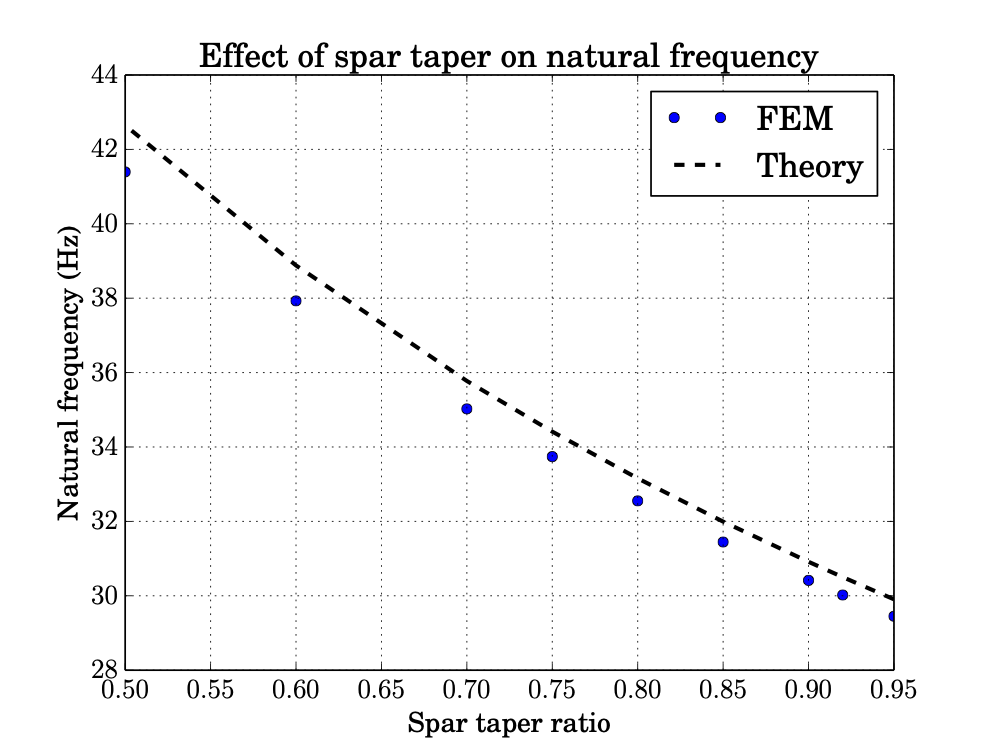
\includegraphics[width=0.45\textwidth]{images/beam_freq1b.png}}
	\subfigure[Rayleigh-Ritz vs. FEM]{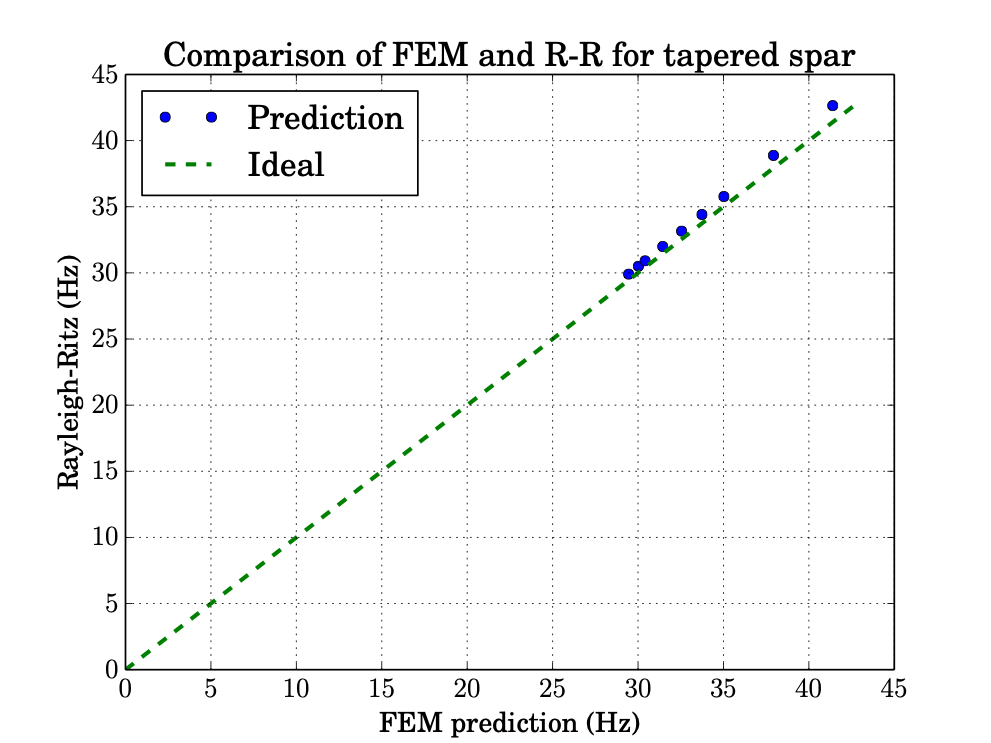
\includegraphics[width=0.45\textwidth]{images/beam_freq1.png}}
     \caption{Natural frequency: Rayleigh-Ritz vs. FEM predicted natural frequencies for a tapered cantilever beam}
     \label{fig:beam_freq1}
\end{figure}

\begin{figure}
     \centering
	\subfigure[Natural frequency vs. taper ratio]{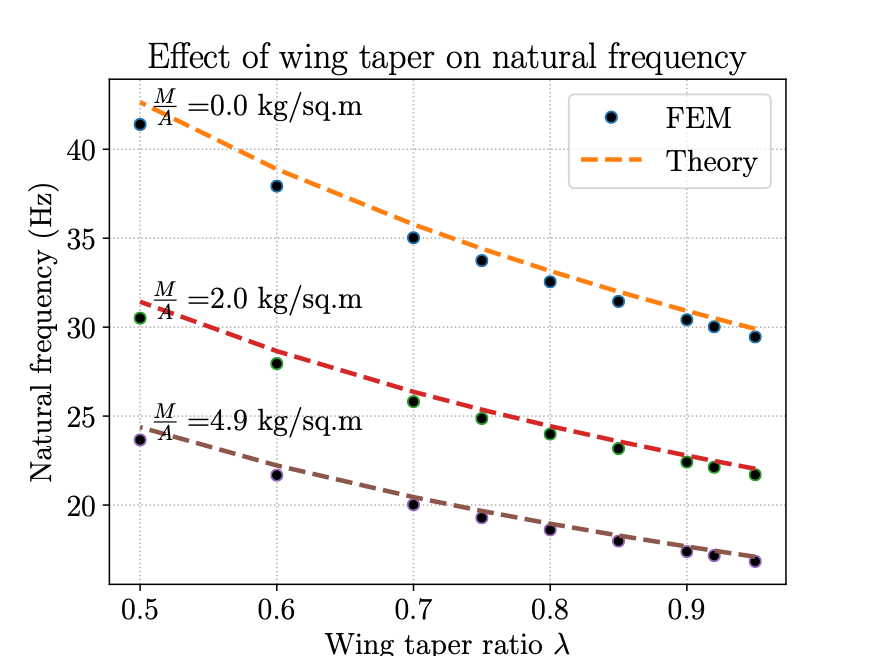
\includegraphics[width=0.45\textwidth]{images/beam_freq2b.png}}
	\subfigure[Rayleigh-Ritz vs. FEM]{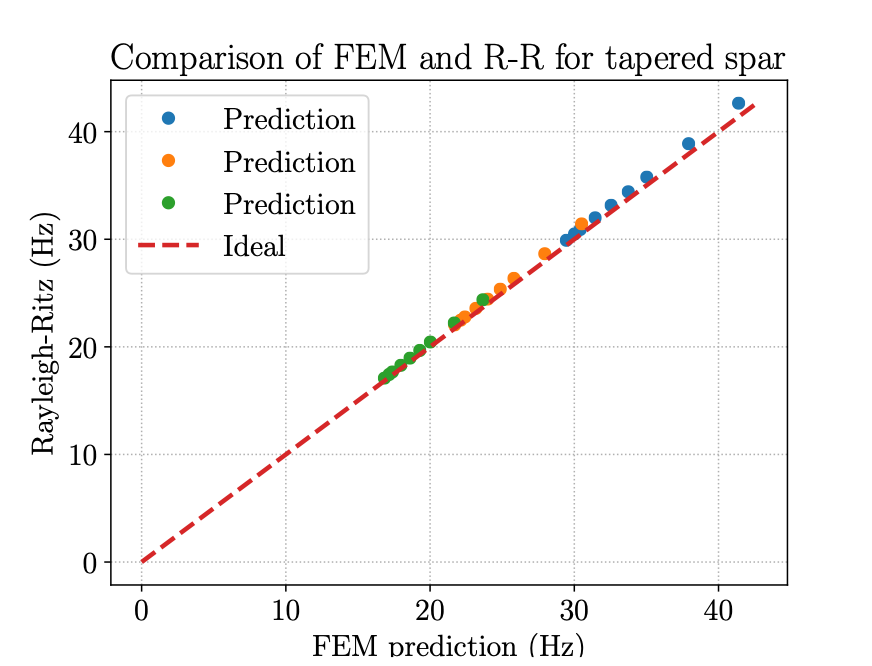
\includegraphics[width=0.45\textwidth]{images/beam_freq2.png}}
     \caption{Natural frequency: Rayleigh-Ritz vs. FEM for a tapered cantilever beam with distributed non-structural masses}
     \label{fig:beam_freq2}
\end{figure}

\subsubsection{Case 2: distributed non-structural mass}
This case is representative of an aircraft half-wing with skin, and no lumped masses. The non-structural masses are represented as a mass per unit area, i.e., $\large\frac{M}{A}$ kg/$m^2$. Three different values of the non-structural mass per unit wing area were evaluated: 0, 2.0 and 4.9 kg/m$^2$. The resulting natural frequencies were calculated from both Rayleigh-Ritz and FEM, and are plotted in Fig.~\ref{fig:beam_freq2}. Excellent agreement is obtained.

\subsubsection{Case 3: half-wing with lumped masses}
This case is representative of an eVTOL wing. The dimensions of the beam are the same as in the previous examples, and the distributed skin mass per unit area is 4.9 kg/m$^2$. Two lumped masses (21.3 kg, 27 kg) are placed along the beam at 0.5$L$ and $L$, respectively. The wing layout and natural frequencies are shown in Fig.~\ref{fig:beam_freq3}.

\begin{figure}
     \centering
	\subfigure[Layout of eVTOL wing]{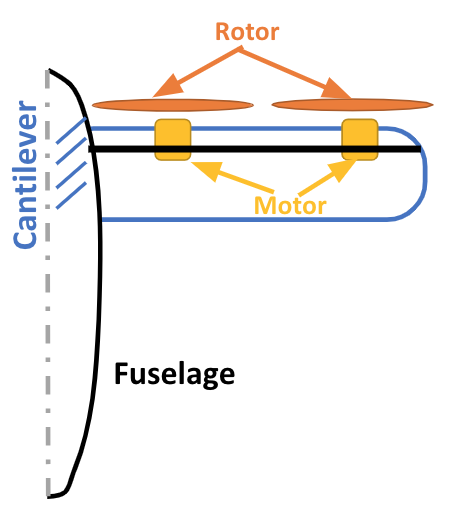
\includegraphics[width=0.3\textwidth]{images/wing_layout.png}}
	\subfigure[Rayleigh-Ritz vs. FEM]{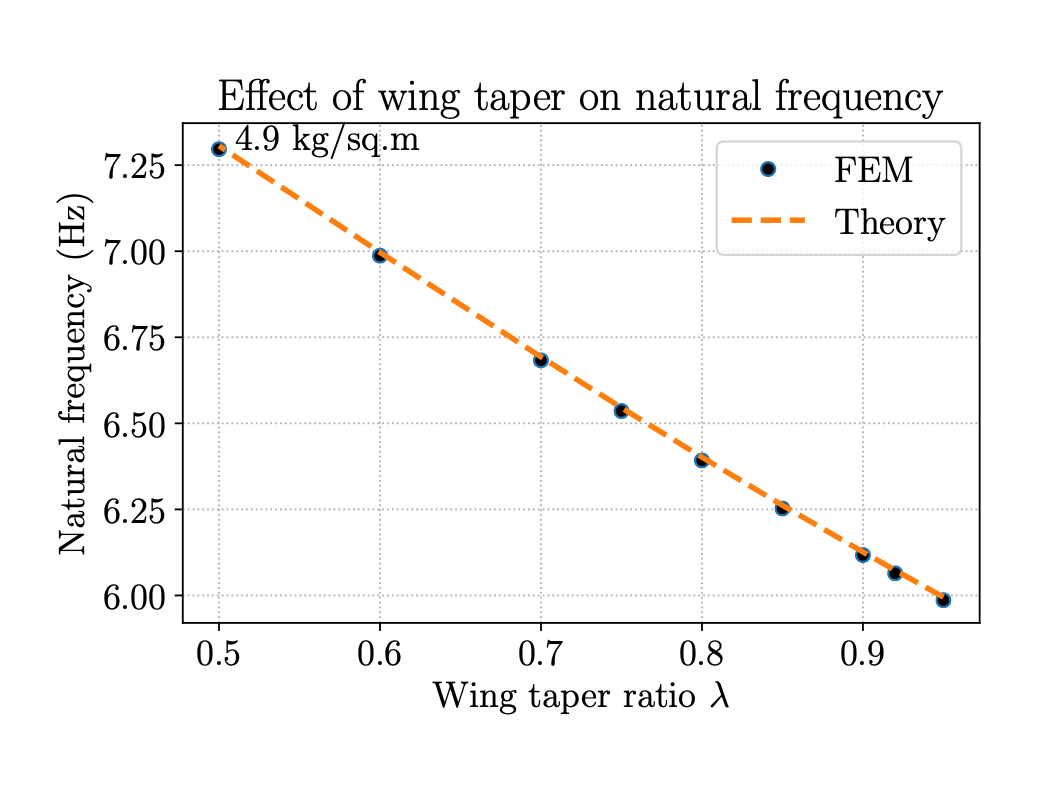
\includegraphics[width=0.45\textwidth]{images/beam_freq3b.png}}
     \caption{Natural frequency: Rayleigh-Ritz vs. FEM for an example eVTOL wing}
     \label{fig:beam_freq3}
\end{figure}